%%% Local Variables: 
%%% mode: latexTeX-master: t
%%% End: 
\documentclass[usenames,dvipsnames]{beamer}
\usepackage{graphicx}
\usepackage{natbib}
%\usepackage[latin1]{inputenc}
%\usepackage[french]{babel}
%\usepackage[T1]{fontenc}
%\usepackage{verbatim}
\usepackage[normalem]{ulem}
\usepackage{amsmath}
%\usepackage{beamerthemeMadrid}
%\usecolortheme{albatross}
%\usepackage{beamerthemeBoadilla} %pas mal du tout
%\usetheme{JuanLesPins}
\usetheme{Madrid}
%\usetheme{Bergen}
\DeclareMathAlphabet{\mathsl}{OT1}{cmss}{m}{sl}
\usepackage{color}
\usepackage{multicol}
%\usepackage{algorithms/algorithm}
%\usepackage{algorithms/algorithmic}
\usepackage{epsfig}
\usepackage{natbib}
\usepackage{graphicx}              % image
%\usepackage{here}                  % positionement facile des figures
%\usepackage[latin1]{inputenc}      % pour les caracteres accentués
%\usepackage[utf8x]{inputenc}
%\usepackage[francais]{babel}
%\usepackage[cyr]{aeguill}  %package permettant la cesure des mots français
%avec utilisation de font T1 avec bon rendu en pdf
%\usepackage[T1]{fontenc}
%\usepackage{lmodern}
\usepackage{fancyhdr}              %gestion entete /pied de pages
\usepackage{amsmath}
\usepackage{amsfonts}
%include pdf page
\usepackage{pdfpages}
\usepackage{fancybox}
\usepackage{pifont}
%\usepackage{multirow}

\usepackage{caption}

\definecolor{brique}{rgb}{0.5,0.2,0.4} 
\definecolor{highlight}{rgb}{1.,0.4,0.}

\newcommand{\RR}{\hbox{\cal I\hspace{-2pt}R}}
\newcommand{\ket}{\right\rangle}       
\newcommand{\bra}{\left\langle}

%\setbeamerfont{frametitle}{series=\bfseries,size=\large,fg=white}
\setbeamerfont{frametitle}{series=\bfseries,size=\large}
\setbeamercolor{structure}{bg=white, fg=brique}

%-------------------------------------------------------------------------------------

\title[hpcscan benchmarks]{hpcscan version 1.2 \\ Performances on various architectures}
%\subtitle{}
%\author[Vincent Etienne]{Vincent Etienne}
%\institute[]{XX}

\date[December 2022] {\small{December 2022}}

%-------------------------------------------------------------------------------------

\bibliographystyle{apalike}


\AtBeginSection[ ]
{
\begin{frame}<beamer>
\frametitle{Content}
\tableofcontents[currentsection]
\end{frame}
}

%\AtBeginSubsection[ ]
%{
%\begin{frame}<beamer>
%\frametitle{Content}
%\tableofcontents[currentsection,currentsubsection]
%\end{frame}
%}

%\titlegraphic{\vspace{-0.75cm} \center
%\pgfimage[height=2.cm]{logo/logo_complet.pdf}}

\begin{document}
\scriptsize

\maketitle 

\clearpage

\frame{
\frametitle{Content}
\tableofcontents }

%*************************************************************************************

\section{Introduction}

%*************************************************************************************

%-------------------------------------------------------------------------------------
\frame{
  \frametitle{Introduction}

  This document presents a characterization of the computing nodes and interconnect on various systems.
  The full set of test cases embedded in \texttt{hpcscan} is used in various configurations.
  
  {\tiny
  \begin{block}{\center List of test cases in this study}

  \begin{table}
    %\caption*{\scriptsize {List of test cases}}
    \label{table_testCases}
    \begin{tabular}{@{}ccc}
      Test Case & Objectives & Remark \\
      \hline
      Memory & Assess memory bandwidth & Scalability analysis on a single node \\
      Grid & Assess bandwidth of grid operations &  Analyse effect of the grid size \\
      Comm & Assess inter-node communication bandwidth & Analyse effect of subdomain decomposition \\
      FD\_D2 & Assess FD spatial derivative computation bandwidth & Analyse effect of FD stencil order \\
      Propa & Find optimal configuration for the wave propagator & Explore range of parameters \\
      Propa & Scalability analysis of wave propagator on multiple nodes & Analyse effect of the FD stencil order \\
    \end{tabular}
  \end{table}
  \end{block}

  \begin{block}{\center General settings}
    \begin{itemize}
    \item All tests are performed in single precision
    \item Best performance is reported over 10 tries for each case (unless stated otherwise)
    \item Grids dimensions are 3D
    \item Grids sizes range from 500 MB up to 4 GB per node
    \item At maximum, 5 grids are allocated (test case Propa) {\bf $\Rightarrow$ max. memory per node is 20 GB}
    \item At maximum, {\bf 8 computing nodes (with one MPI proc per node) are used}
    \end{itemize}
  \end{block}
  }
  }
%-------------------------------------------------------------------------------------

%*************************************************************************************

\section{Presentation of the systems}

%*************************************************************************************


%*************************************************************************************

\subsection{NEC SX-Aurora}

%*************************************************************************************

%-------------------------------------------------------------------------------------
\frame{
  \frametitle{NEC SX-Aurora}

  \begin{block}{\center NEC SX-Aurora}

  \scriptsize
  \begin{itemize}
  \item XX
  \end{itemize}

  \end{block}

  \begin{figure}
    \begin{center}
      
\includegraphics[width=0.5 \textwidth]{./Images/InProgress.jpg}
    \end{center}
  \end{figure}
}

%*************************************************************************************

\section{Test Case Memory}

%*************************************************************************************

%-------------------------------------------------------------------------------------
\frame{
  \frametitle{Test Case Memory - Description}

  \begin{block}{\center Benchmark objective}
    \textcolor{Sepia}{\bf Assess memory bandwidth}
    \begin{itemize}
    \item Measure GByte/s and GPoint/s for simple operations on memory arrays
    \item Scalability analysis on a single node
    \item Get a reference to compare with for the following tests
  \end{itemize}
  \end{block}

  \begin{block}{\center Benchmark configuration}
    \begin{itemize}
    \item Scalability on 1 node with 1 to max number of threads (cores) on the node
    \item Array size 4 GB
    \item Reproduce results with \texttt{./script/testCase\_Memory/hpcscanMemory.sh}
    \item Elapsed time less than 5 minutes
    \end{itemize}
  \end{block}
}

%-------------------------------------------------------------------------------------
\frame{
  \frametitle{Test Case Memory - NEC SX-Aurora TSUBASA 20B \footnote{\scriptsize \textcolor{blue}{Results updated Dec 23, 2022}} }

  \center{\bf TestMode Baseline}
  
  \begin{figure}
    \begin{center}
      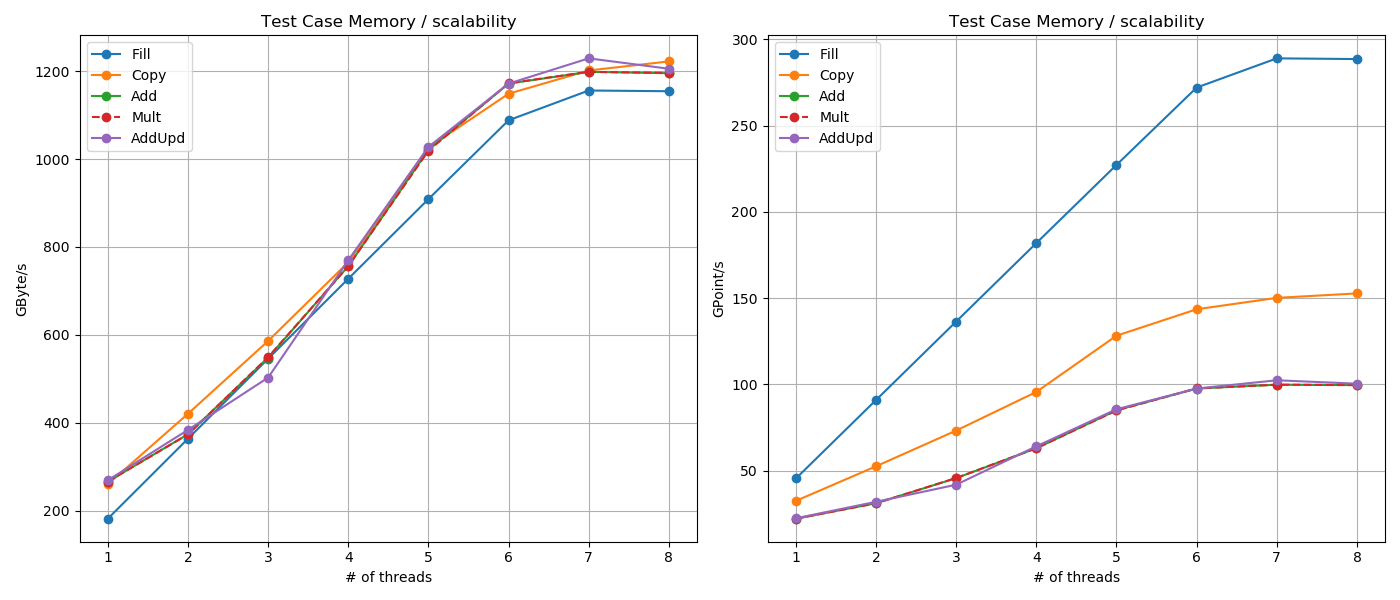
\includegraphics[width=1.0 \textwidth]{../../script/testCase_Memory/hpcscanPerfMemoryProto27.png}
    \end{center}
  \end{figure}
}

%*************************************************************************************

\section{Test Case Grid}

%*************************************************************************************

%-------------------------------------------------------------------------------------
\frame{
  \frametitle{Test Case Grid - Description}

  \begin{block}{\center Benchmark objective}
    \textcolor{Sepia}{\bf Assess bandwidth of grid operations}
    \begin{itemize}
    \item Measure GByte/s and GPoint/s for simple and complex operations on 3D grids
    \item Analyse effect of the grid size
    \end{itemize}
  \end{block}

  \begin{block}{\center Benchmark configuration}
    \begin{itemize}
    \item 1 node with max number of threads (cores) on the node
    \item 2 grid sizes
      \begin{itemize}
      \item \scriptsize Small size 500 MB (500 x 500 x 500 points)
      \item \scriptsize Medium size 4 GB (1000 x 1000 x 1000 points)
      \end{itemize}
    \item Reproduce results with \texttt{./script/testCase\_Grid/hpcscanGrid.sh}
    \item Elapsed time less than 5 minutes
    \end{itemize}
  \end{block}
  
}

%-------------------------------------------------------------------------------------
\frame{
  \frametitle{Test Case Grid - NEC SX-Aurora TSUBASA 20B \footnote{\scriptsize \textcolor{blue}{Results updated Dec 23, 2022}} }

  \center{\bf TestMode Baseline}
  
  \begin{figure}
    \begin{center}
      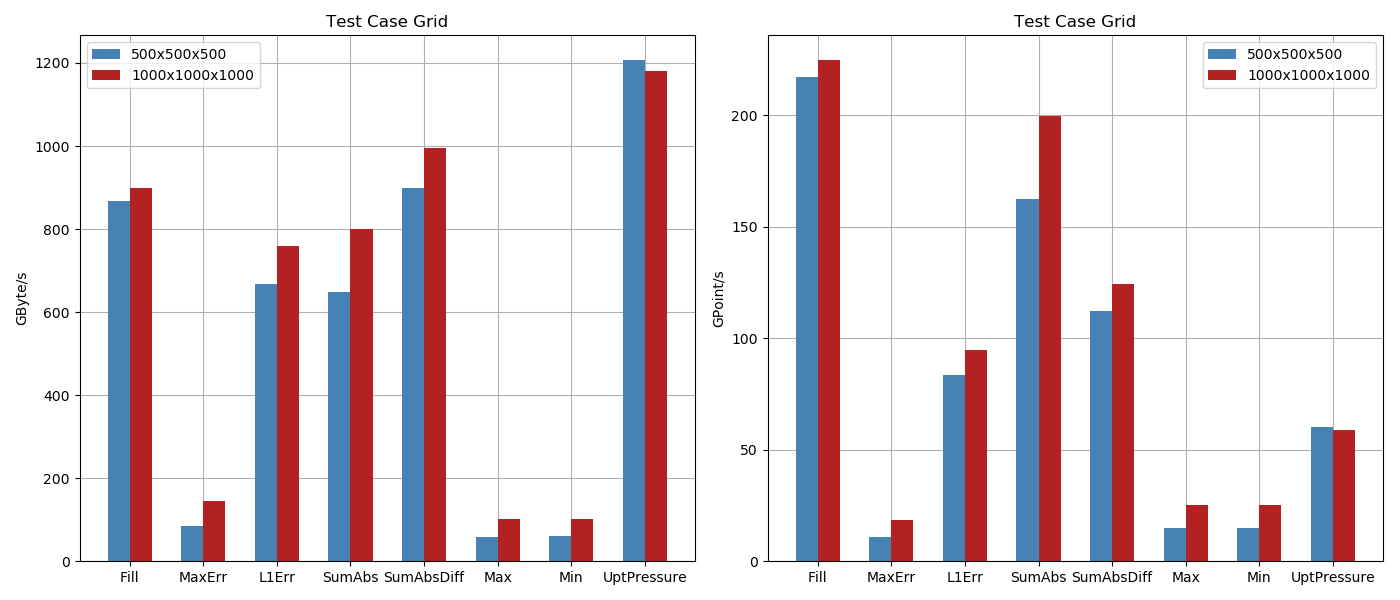
\includegraphics[width=1.0 \textwidth]{../../script/testCase_Grid/hpcscanPerfGridProto27Baseline.png}
    \end{center}
  \end{figure}

  ApplyBoundaryCondition performs at 317/538 GBytes (39.6/67.2 Gpoint/s)
}

%-------------------------------------------------------------------------------------
\frame{
  \frametitle{Test Case Grid - NEC SX-Aurora TSUBASA 20B \footnote{\scriptsize \textcolor{blue}{Results updated Dec 23, 2022}} }

  \center{\bf TestMode NEC}
  
  \begin{figure}
    \begin{center}
      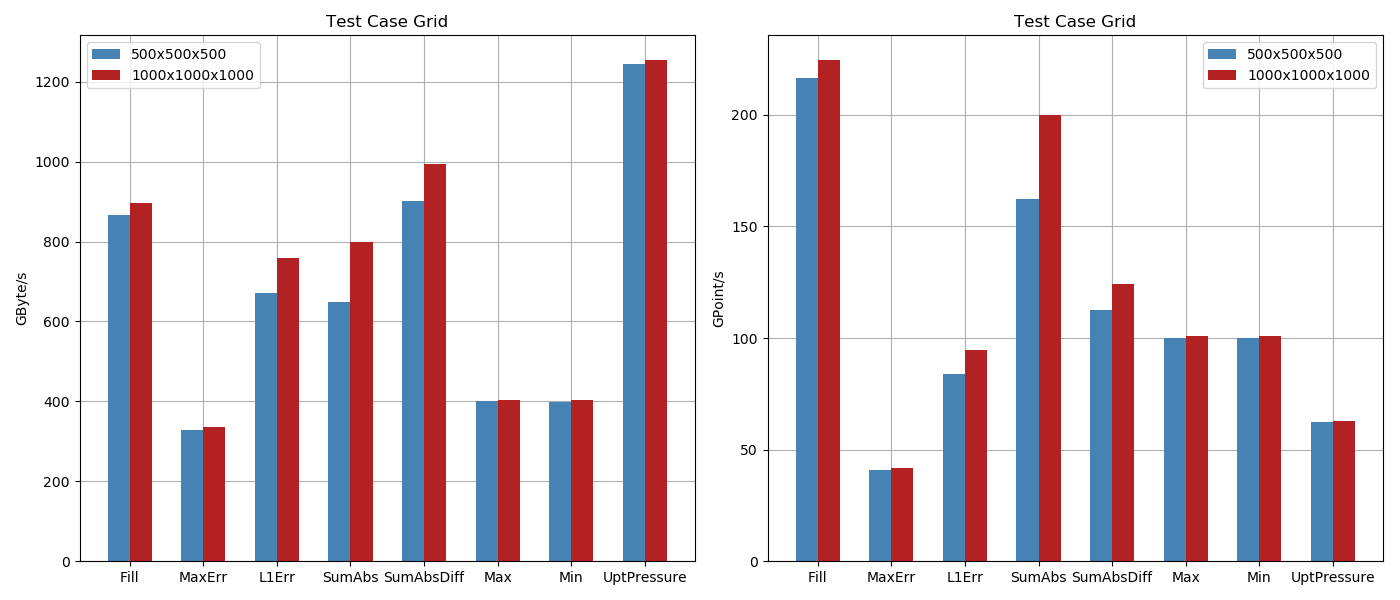
\includegraphics[width=1.0 \textwidth]{../../script/testCase_Grid/hpcscanPerfGridProto27NEC.png}
    \end{center}
  \end{figure}

  ApplyBoundaryCondition performs at 3437/6502 GBytes (429/813 Gpoint/s)
}

%*************************************************************************************

\section{Test Case Comm}

%*************************************************************************************

%-------------------------------------------------------------------------------------
\frame{
  \frametitle{Test Case Comm - Description}

  \begin{block}{\center Benchmark objective}
    \textcolor{Sepia}{\bf Assess inter-node communication bandwidth}
  
    \vspace{0.25cm}
    Point to point communication
    \begin{itemize}
    \item Half-duplex BW with MPI\_Send from proc X to proc 0
    \item Full-duplex BW with MPI\_Sendrecv between proc X and proc 0
    \end{itemize}

    Collective communication
    \begin{itemize}
    \item Grid halos exchange (used in FD kernels) with MPI\_Sendrecv
    \item Analyse effect of subdomain decomposition geometry
    \end{itemize}
  \end{block}

  \begin{block}{\center Benchmark configuration}
    \begin{itemize}
    \item 8 nodes with 1 MPI/node \& 32 threads/node
    \item Baseline kernel
    \item Grid size 4 GB (1000 x 1000 x 1000 points)
    \item FD order O8
    \item Subdomain decomposition: 1x4x2, 1x2x4 \& 2x2x2
    \item Reproduce results with \texttt{./script/testCase\_Comm/hpcscanComm.sh}
    \item Total 3 configurations: Elapsed time less than 1 minute
    \end{itemize}
  \end{block}
}


%-------------------------------------------------------------------------------------
\frame{
  \frametitle{Test Case Comm - NEC SX-Aurora TSUBASA XX \footnote{\scriptsize \textcolor{blue}{Updated Dec XX, 2022}} }

  \begin{figure}
    \begin{center}
      %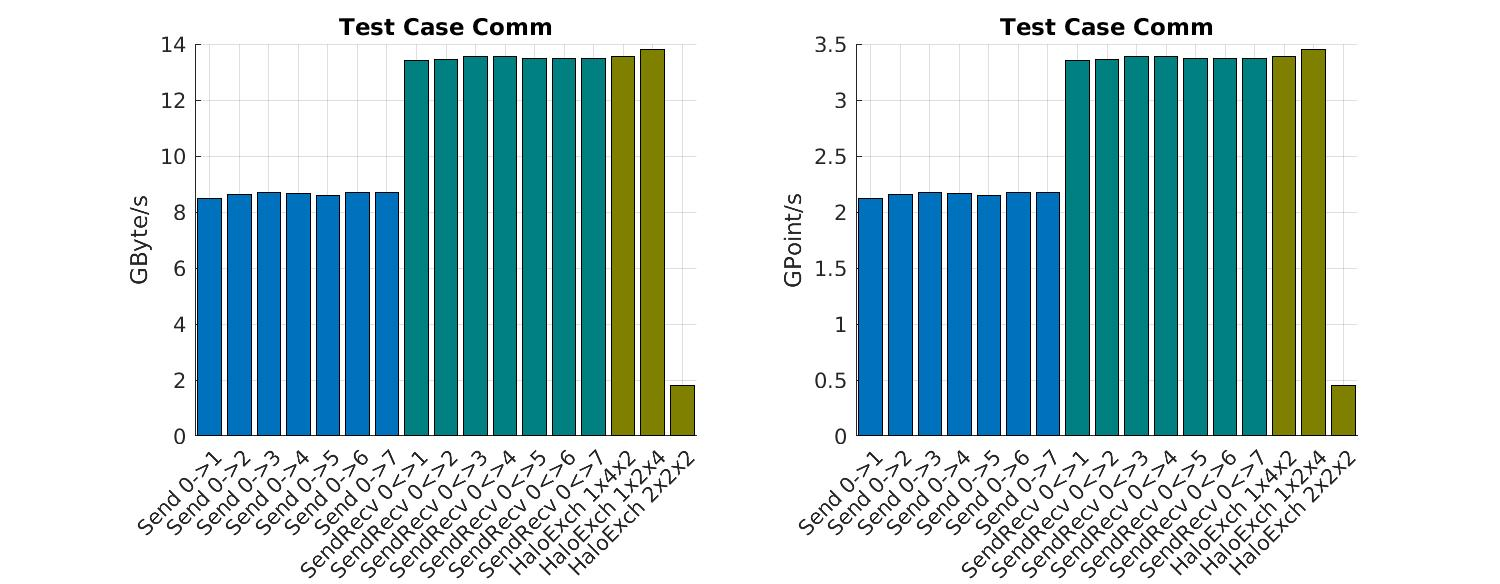
\includegraphics[width=1.0 \textwidth]{../../script/testCase_Comm/hpcscanCommShaheen.jpg}
      
\includegraphics[width=0.5 \textwidth]{./Images/InProgress.jpg}
    \end{center}
  \end{figure}

}

%*************************************************************************************

\section{Test Case FD\_D2}

%*************************************************************************************

%-------------------------------------------------------------------------------------
\frame{
  \frametitle{Test Case FD\_D2 - Description}

  \begin{block}{\center Benchmark objective}
    \textcolor{Sepia}{\bf Assess FD spatial derivative computation bandwidth}
    \begin{itemize}
    \item Directionnal derivatives
      \begin{itemize}
      \item {\tiny Axis 1, $W = \partial^2_{x1} (U)$}
      \item {\tiny Axis 2, $W = \partial^2_{x2} (U)$}
      \item {\tiny Axis 3, $W = \partial^2_{x3} (U)$}
      \end{itemize}
    \item Laplacian $W = \Delta (U)$
    \item Analyse effect of FD stencil order
    \item Try different implementations of FD computation
    \end{itemize}
  \end{block}

  \begin{block}{\center Benchmark configuration}
    \begin{itemize}
    \item 1 node with 32 threads
    \item 2 test modes: Baseline \& CacheBlk
    \item Grid size 4 GB (1000 x 1000 x 1000 points)
    \item FD orders 2, 4, 8, 12 \& 16
    \item Reproduce results with \texttt{./script/testCase\_FD\_D2/hpcscanFD\_D2.sh}
    \item Total 10 configurations: Elapsed time about 2 minutes
    \end{itemize}
  \end{block}
}

%-------------------------------------------------------------------------------------
\frame{
  \frametitle{Test Case FD\_D2 - NEC SX-Aurora TSUBASA XX \footnote{\scriptsize \textcolor{blue}{Updated Dec XX, 2022}} }

  \begin{figure}
    \begin{center}
      %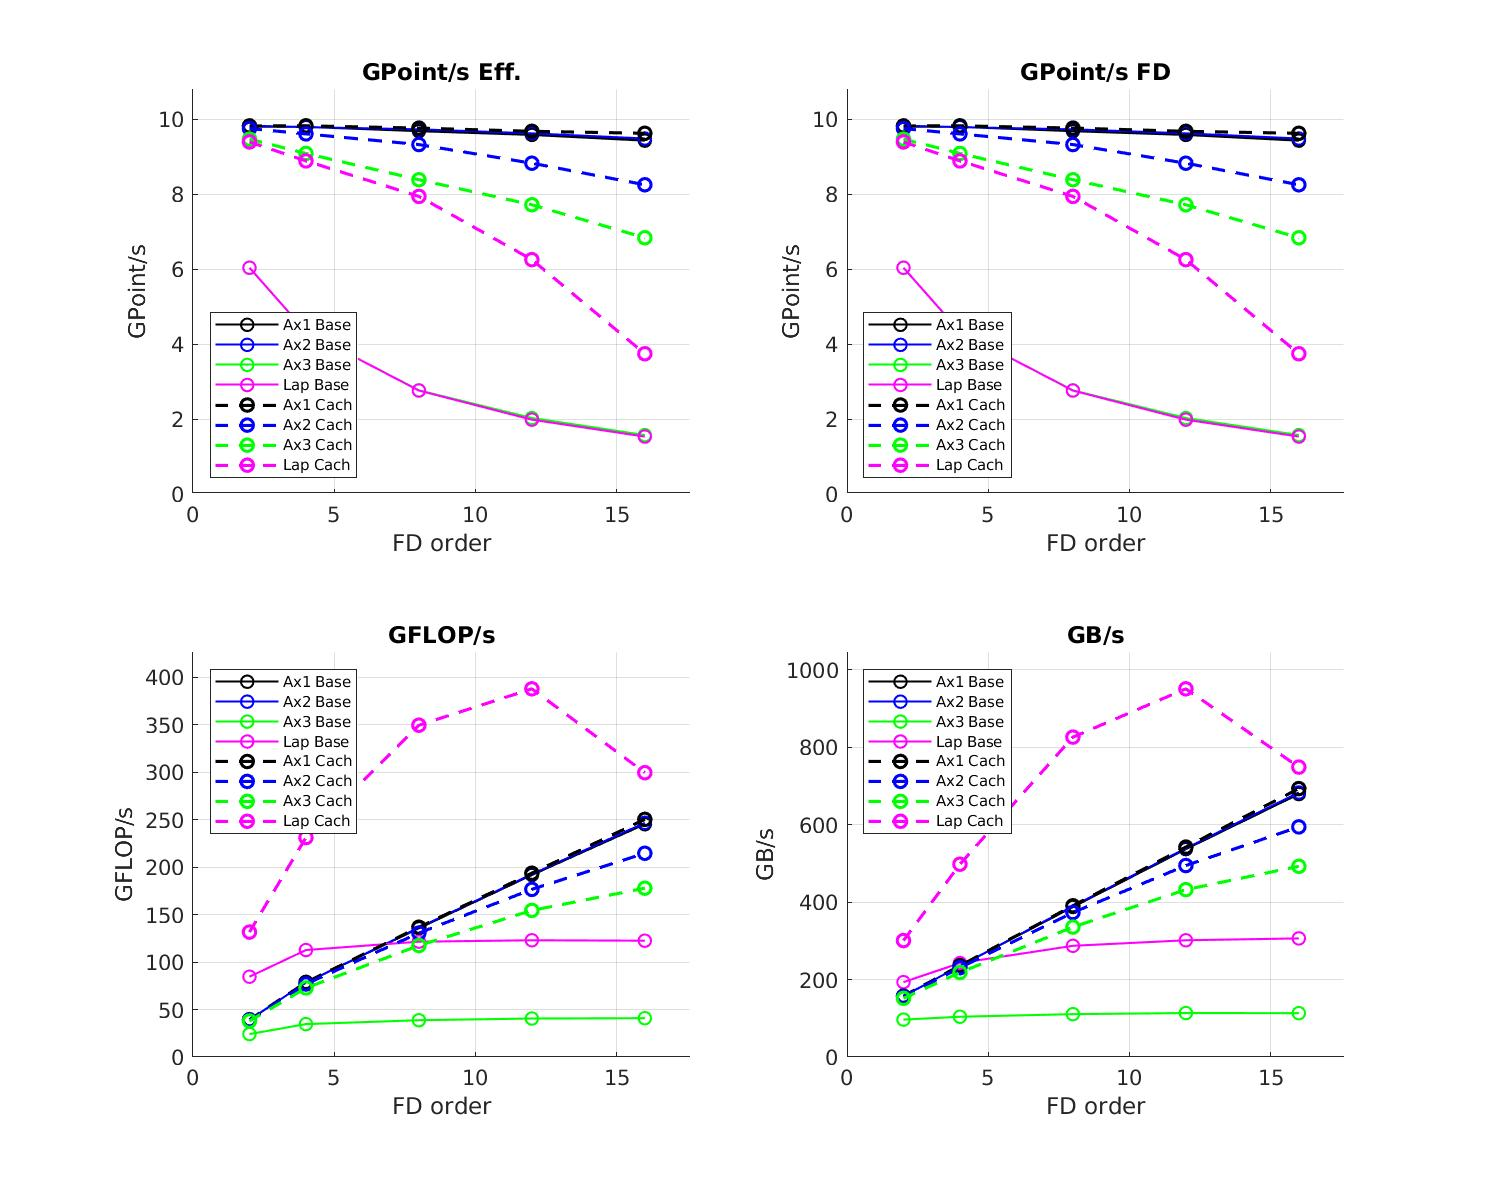
\includegraphics[width=0.8 \textwidth]{../../script/testCase_FD_D2/hpcscanFD_D2Shaheen.jpg}
      
\includegraphics[width=0.5 \textwidth]{./Images/InProgress.jpg}
    \end{center}
  \end{figure}
}

%*************************************************************************************

\section{Test Case Propa}

%*************************************************************************************

%-------------------------------------------------------------------------------------
\frame{
  \frametitle{Test Case Propa - Description}

  \begin{block}{\center Benchmark objective}
    \textcolor{Sepia}{\bf Find optimal configuration for the wave propagator regarding accuracy/cost}
    \begin{itemize}
    \item Physical problem: 3D domain, size 130 $\lambda$ in all direction, tmax = 11 periods
    \item Explore range of grid sampling and time step
    \item Explore range of FD order
    \item Try different implementations of the propagator
    \end{itemize}
    
  \end{block}

  \begin{block}{\center Benchmark configuration}
    \begin{itemize}
    \item 1 node with 32 threads
    \item Test mode CachBlk
    \item 2 propagator implementations: Ac2Standard and Ac2SplitComp
    \item FD orders 4, 8 \& 12
    \item Time step 100, 50 and 10\% of stability time step
    \item Grid size from 500x500x500 (500 MB) to 1000x1000x1000 (4 GB)
    \item nt from 101 to 2311 (depending of the configuration) \& ntry = 4
    \item Reproduce results with \texttt{./script/testCase\_Propa/paramAnalysis/hpcscanPropaParamAnalysis.sh}
    \item Total 108 configurations: Elapsed time about 12 hours
    \end{itemize}
  \end{block}
}

%-------------------------------------------------------------------------------------
\frame{
  \frametitle{Test Case Propa - NEC SX-Aurora TSUBASA XX \footnote{\scriptsize \textcolor{blue}{Updated Dec XX, 2022}} }

  \center \tiny Blue=FD O4, Pink=FD O8,Red=FD O12 / Square=Ac2Standard, Cross=Ac2SplitComp
  
   \begin{figure}
    \begin{center}
      %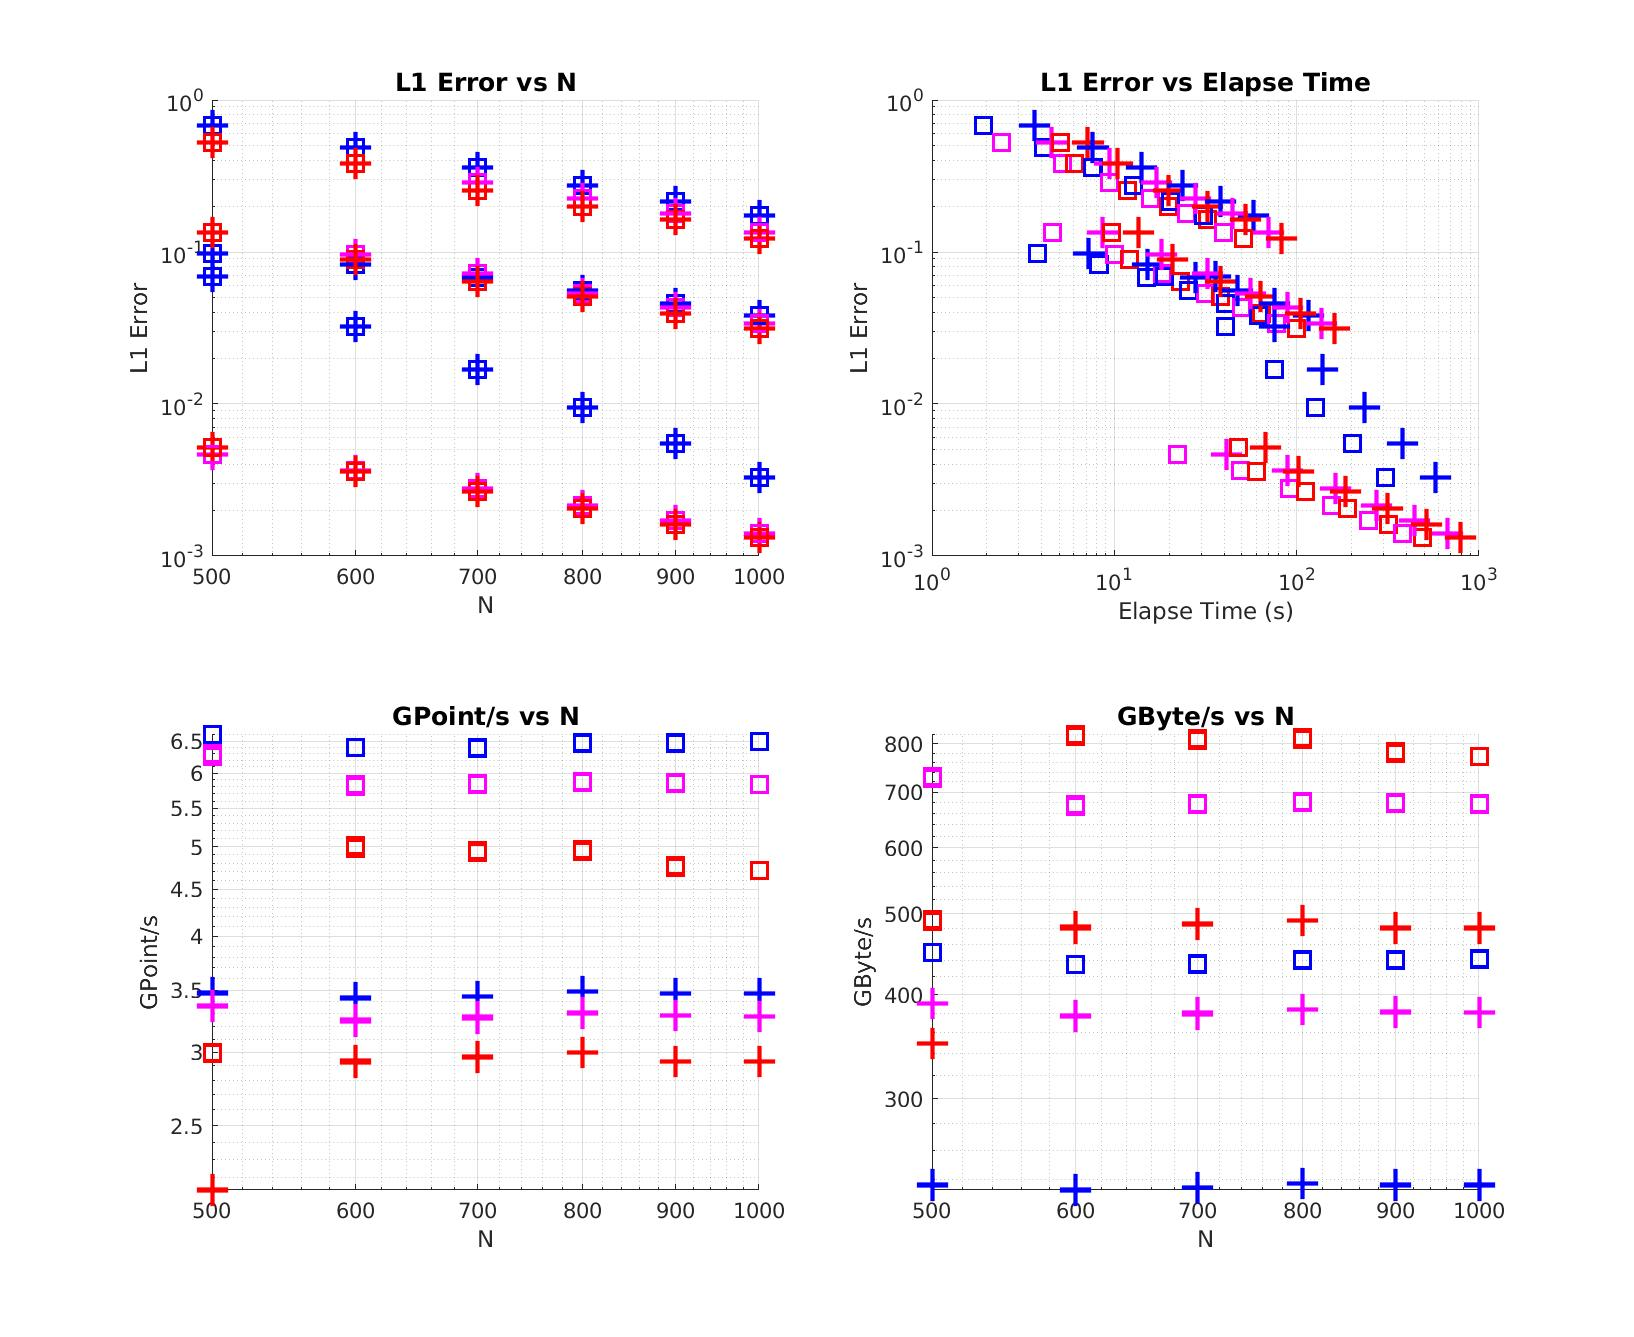
\includegraphics[width=0.7 \textwidth]{../../script/testCase_Propa/paramAnalysis/hpcscanPropaParamAnalysisShaheen.jpg}
      
\includegraphics[width=0.5 \textwidth]{./Images/InProgress.jpg}
    \end{center}
  \end{figure}

}

%-------------------------------------------------------------------------------------
\frame{
  \frametitle{Test Case Propa - Description}

  \begin{block}{\center Benchmark objective}
    \textcolor{Sepia}{\bf Scalability analysis of the wave propagator on multiple nodes}
    \begin{itemize}
    \item Strong and weak scalability
    \item Analyse effect of the FD stencil order
    \end{itemize}
    
  \end{block}

  \begin{block}{\center Benchmark configuration}
    \begin{itemize}
    \item From 1 node to 8 nodes with 32 threads/node
    \item Test mode CachBlk (best config from test case FD\_D2)
    \item Propagator implementation Ac2Standard (best config from previous test case)
    \item FD orders 4, 8 \& 12
    \item Subdomain decomposition geometry is best config obtained in test case Comm
    \item Strong scalability: Grid size 1000x1000x1000 (4 GB)
    \item Weak scalability: Grid size from 1000x1000x1000 (4 GB) to 1000x4000x2000 (32 GB)
    \item nt = 100
    \item Reproduce results with \texttt{./script/testCase\_strongWeakScalability/hpcscanPropaStrongWeakScalability.sh}
    \item Total 30 configurations: Elapsed time about 1h 15min
    \end{itemize}
  \end{block}
}


%-------------------------------------------------------------------------------------
\frame{
  \frametitle{Test Case Propa - NEC SX-Aurora TSUBASA XX \footnote{\scriptsize \textcolor{blue}{Updated Dec XX, 2022}} }

  \begin{figure}
    \begin{center}
      %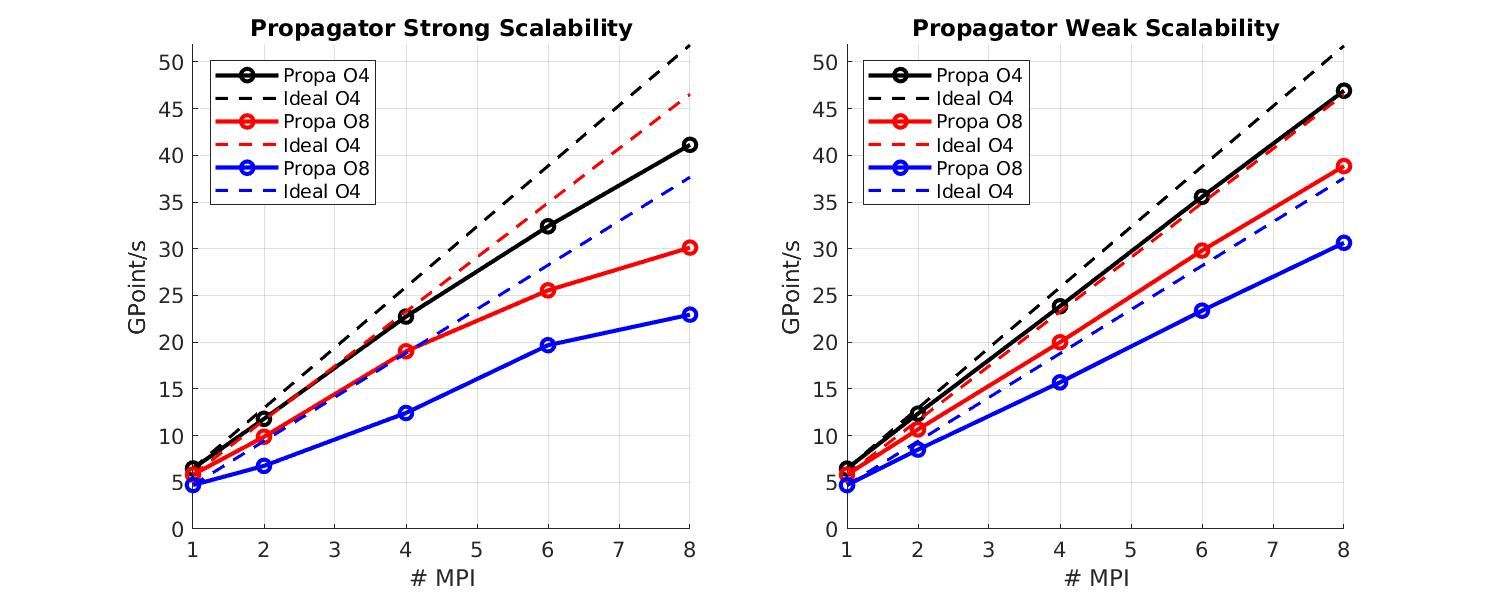
\includegraphics[width=1.0 \textwidth]{../../script/testCase_Propa/strongWeakScalability/hpcscanPropaStrongWeakScalabilityShaheen.jpg}
      
\includegraphics[width=0.5 \textwidth]{./Images/InProgress.jpg}
    \end{center}
  \end{figure}
}

%*************************************************************************************

\section{Summary}

%*************************************************************************************

%-------------------------------------------------------------------------------------
\frame{
  \frametitle{Summary}

  \begin{block}{\center Test Case Memory}
    \begin{itemize}
    \item Highest memory BW for Add+Update 118 GB/s [9.8 GPoint/s] (86 \% of peak BW)
    \item Lowest memory BW for Fill 54 GB/s [13.5 GPoint/s] (40 \% of peak BW)
    \item All cores (32 threads) are required to reach best perf. on the node
    \end{itemize}
  \end{block}

  \begin{block}{\center Test Case Grid}
    \begin{itemize}
    \item Highest memory BW for L1Err, SumAbs, SumAbsDiff, GetMin \& GetMax 125 GB/s (92 \% of peak BW)
    \item In terms of GPoint/s: 15 for L1Err \& SumAbsDiff and 30 for SumAbs, GetMin \& GetMax
    \item Lowest memory BW for Fill 54 GB/s [13.5 GPoint/s] (40 \% of peak BW)
    \item Minor effect of the grid size on the performance
    \item Results are consistent with the test case Memory
    \end{itemize}
  \end{block}
  }
%-------------------------------------------------------------------------------------

%-------------------------------------------------------------------------------------
\frame{
  \frametitle{Summary}

  \begin{block}{\center Test Case Comm}
    \begin{itemize}
    \item Half-duplex BW about 8.6 GByte/s [2.1 GPoint/s]
    \item Full-duplex BW about 13.4 GByte/s [3.3 GPoint/s]
    \item Communication BW is similar between 8 nodes (no unbalance observed)
    \item Grid halos exchange: large effect of subdomain decomposition geometry
      \begin{itemize}
      \item \scriptsize Best BW: 1x4x2 or 1x2x4 with 13.6 GByte/s [3.4 GPoint/s]
      \item \scriptsize Worst BW: 2x2x2 with 1.8 GByte/s [0.5 GPoint/s]
      \end{itemize}
    \end{itemize}
  \end{block}
}
%-------------------------------------------------------------------------------------

%-------------------------------------------------------------------------------------
\frame{
  \frametitle{Summary}
  
  \begin{block}{\center Test Case FD\_D2}
    \begin{itemize}
    \item Max. 10 GPoint/s for $\partial^2_{x1}$ for all FD orders
    \item Large effect of Cache Blocking
      \begin{itemize}
      \item \scriptsize Max 950 GByte/s for $\Delta$ O12 with Cache Blocking (x7 memory BW)
      \item \scriptsize Max 300 GByte/s for $\Delta$ O12 Baseline (speed-up 3.2 with Cache Blocking)
      \item \scriptsize GFlop/s increases for all derivatives with the FD order (except for $\Delta$ O16)
      \item \scriptsize Cache Block size is n2=4, n3=16 and full size for n1 (optimized for Shaheen \footnote{\tiny \textcolor{blue}{Etienne, V., et al. "High-performance seismic modeling with finite-difference using spatial and temporal cache blocking." Third EAGE Workshop on High Performance Computing for Upstream. Vol. 2017. No. 1. European Association of Geoscientists \& Engineers, 2017.}})
      \end{itemize}
    \item Max. 390 GFlop/s for $\Delta$ O12 with Cache Blocking (17 \% peak GFlop/s)
    \item Lowest GFlop/s observed for  $\partial^2_{x3}$
    \end{itemize}
  \end{block}
}
%-------------------------------------------------------------------------------------

%-------------------------------------------------------------------------------------
\frame{
  \frametitle{Summary}

  \begin{block}{\center Test Case Propa - Parametric analysis}

    \begin{itemize}
    \item Accuracy
      \begin{itemize}
      \item \scriptsize Increases with FD orders, number of grid points and number of time steps
      \item \scriptsize Stability time step is too large for high order FD stencils to reach optimal convergence
      \end{itemize}
    \item Optimal config to reach error less than 1\% with minimal elapsed time
      \begin{itemize}
      \item \scriptsize FD O8 - Cache Blocking - Standard propagator implementation with N=500 and 10\% stability time step
      \item \scriptsize This schemes perform at 6.2 GPoint/s and 720 GByte/s (elapsed time 22 s)
      \item \scriptsize To reach similar accuracy, FD O4 requires N=900 and an elapsed time 203 s (9.2 times longer than O8)
      \end{itemize}
    \item Implementation algorithm
      \begin{itemize}
      \item \scriptsize Splitting computation with a separate Laplacian computation slows down the propagator by 2
      \end{itemize}
    \end{itemize}

  \end{block}
}
%-------------------------------------------------------------------------------------

%-------------------------------------------------------------------------------------
\frame{
  \frametitle{Summary}

  \begin{block}{\center Test Case Propa - Scalability}
    
    \begin{itemize}
    \item Strong scalability
      \begin{itemize}
      \item \scriptsize Speed-up is sub-linear and gets worst as the number of nodes increases
      \item \scriptsize Parallel efficiency decreases with FD order
      \item \scriptsize Parallel efficiency on 8 nodes: 77\% for O4, 64\% for O8 and 60\% for O12
      \end{itemize}
    \item Weak scalability
      \begin{itemize}
      \item \scriptsize Speed-up is linear
      \item \scriptsize Parallel efficiency decreases with FD order
      \item \scriptsize Parallel efficiency on 8 nodes: 90\% for O4, 83\% for O8 and 80\% for O12
      \end{itemize}
    \end{itemize}
    
  \end{block}
}
%-------------------------------------------------------------------------------------

%*************************************************************************************

\section{Acknowledgements}

%*************************************************************************************

%-------------------------------------------------------------------------------------
\frame{
  \frametitle{Acknowledgements}
  \begin{itemize}
  \item XX
  \end{itemize}
}

%-------------------------------------------------------------------------------------
%{\tiny{
%\def\newblock{\hskip .11em plus .33em minus .07em}
%\bibliographystyle{apalike}
%\bibliography{./biblioseiscope}
%}}

%\addtocounter{framenumber}{-4}

\end{document}

